\documentclass[a4paper,10pt]{article}
\usepackage[utf8]{inputenc}
\usepackage{charter}
\usepackage{listings}
\usepackage{color}
\usepackage{url}
\usepackage{amssymb}
\usepackage{amsmath}
\usepackage{hyperref}
\usepackage{graphicx}
\usepackage{float}
%\usepackage[section]{placeins}

\definecolor{grey}{rgb}{0.9,0.9,0.9}

\lstset{
language=Python,
basicstyle=\footnotesize\fontfamily{pcr},
backgroundcolor=\color{grey},
numbers=left,
numberstyle=\tiny,
numbersep=5pt,
showstringspaces=false,
tabsize=2,
breaklines=true
}

\setlength{\parindent}{0pt}

\title{Improving schedulability rate of EDF when taking into account the preemption cost in uniprocessor periodic systems}
\author{Thomas Chapeaux}
\date{Summer 2013}
%opening
\sloppy
\begin{document}
\maketitle

\tableofcontents

\newpage

\begin{abstract}

In preemptive scheduling techniques of real-time systems, a task can be interrupted during its execution to allow another task to meet its deadline. Previous results, such as the optimality of the EDF scheduler, assume that the added cost of the preemptions (including context saving and restoration, as well as the increase in cache misses) is negligible compared to the tasks execution times. In this paper, we show that within a model taking this cost into account, the optimality of EDF is no longer guaranteed. We then propose another algorithm which strictly dominates EDF in the model, and prove that it is also optimal for implicit deadline systems.

\end{abstract}

\newpage

\section{Introduction}

...

\section{Model}

    \subsection{State of the Art}

        The results presented in this section use the assumption that preemption times are negligible.\\

        We use an extension of Liu and Layland model presented in \cite{Liu:2000:RS:518501} to formalize real-time systems. This model represents such systems by a set of \textbf{tasks} generating \textbf{jobs}, where a job is a whole entity of computation with a given time of arrival and a given deadline.

        \subsubsection{Tasks and jobs}

        Tasks are used to model recurring jobs. They are denoted as the tuple $\tau_i = (O_i, T_i, D_i, C_i)$, where
        \begin{itemize}
            \item $i = \{1,2,...\}$ is an unique identifier for the task.
            \item $O_i$ is the minimal time at which the first job of the tasks is generated.
            \item $T_i$ is the minimal time between two job generations.
            \item $D_i$ is the relative deadline of its job.
            \item $C_i$ is the execution time of its job.
        \end{itemize}

        A task $\tau_i$ generates jobs, denoted as the tuple $J_{i,j} = (a_{i, j}, d_{i,j}, c_{i,j})$ where :
        \begin{itemize}
            \item $j = \{1,2,...\}$ is an unique identifier for the job within $\tau_i$.
            \item $a_{i,j} = O_i + (j-1) \cdot T_i$ is the arrival time (or \emph{activation time}) of the job.
            \item $d_{i,j} = a_{i,j} + D_i$ is an absolute deadline at which the job must be completed.
            \item $c_{i,j} = C_i$ is the time it takes to complete the job (\emph{execution time}).
        \end{itemize}

        We also assume a discrete time, meaning that we consider that time passes one unit (sometimes called \emph{clock tick}) at a time. This means that the values listed above must be integers and that jobs will execute for whole units.\\

        In this paper, we only consider \textbf{constrained deadline} systems, where $D_i \leqslant T_i \; \forall i$, and sometimes the particular case of \textbf{implicit deadline} systems, where $D_i = T_i$.\\

        Similarly, we differentiate between \textbf{synchronous system} (where $O_i = O_j \; \forall i,j$) and asynchronous systems (which are not synchronous).\\

        To summarize, Fig.~\ref{fig:rt_ex} shows an example of real-time system in our model.

        \begin{figure}[H]
        \begin{center}
            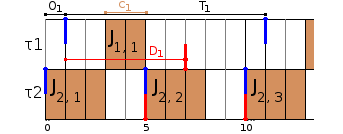
\includegraphics{figs/RTsystem_example.png}
            \caption{A task system. Annotations will be removed in later figures}
            \label{fig:rt_ex}
        \end{center}
        \end{figure}


        \subsubsection{Schedule and feasibility}

        A scheduling policy (or \emph{algorithm}) is said to be \textbf{idling} if it allows instants at which no jobs are executing even if there are released and unfinished jobs present in the system. It is said to be \textbf{preemptive} if it allows the processor to begin computation of a new job when the currently computed job is still unfinished.\\

        A system is said to be \textbf{schedulable by a scheduling policy} if it exists a scheduling policy such that every job in the task set completes before its deadline is reached. A system schedulable by at least one scheduling policy is said to be \textbf{feasible}.\\

        The authors of \cite{liu1973scheduling} have shown that the EDF (Earliest Deadline First) scheduling policy, in which jobs are prioritized according to their absolute deadline, is optimal, meaning that any feasible system is schedulable by EDF.

        \subsubsection{Feasibility Analysis}

        For implicit task systems, $U_{tot} \leqslant 1$ is a necessary and sufficient condition of feasibility.\\

        For (a)synchronous constrained deadline systems, $[O_{max}, O_{max} + 2 \cdot H]$ (with $O_{max}$ being the maximal task offset and $H$ the LCM of periods) is a feasibility interval for EDF.

    \subsection{Preemption Cost}

        We now consider that preemption costs are not negligible. We thus define a parameter $\alpha$, constant for all tasks of a system, called the preemption cost.\\

        Once a previously preempted job is chosen for computation by the scheduling policy, it enters an uninterruptible preemption recovery period, as seen in Fig.~\ref{fig:prp}.\\

        \begin{figure}[H]
        \begin{center}
            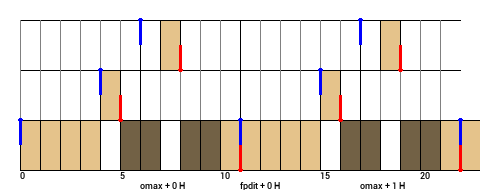
\includegraphics[width=\textwidth]{figs/atomicpreemption_example.png}
            \caption{Schedule of a system with $\alpha=2$. At t $t=6$, the preemption recovery period is not interrupted even though a job with higher priority is activated}
            \label{fig:prp}
        \end{center}
        \end{figure}

        The authors of \cite{meumeu2007extending} (TOCHECK) propose an unnamed (we use PA-RMA to refer to it) fixed-priority-optimal scheduling policy for synchronous implicit deadline systems.

\section{Performance of EDF with preemption cost}
% Rename section to something like "Old results do not hold, bitch"

    In this section, we show that the EDF scheduling policy, optimal when the preemption costs are negligible, is less adapted to our model with costly preemptions.

    \subsection{Non-optimality}

        Consider the following task system

        \begin{center}
            \begin{tabular}{|r|c|c|c|c|c|}
                \hline
                            & $O_i$ & $C_i$ & $D_i$ & $T_i$ & $\alpha_i$ \\ \hline
                $\tau_1$    & 0     & 3     & 6    & 6     & 2     \\ \hline
                $\tau_2$    & 1     & 2     & 4    & 4     & 2     \\ \hline
            \end{tabular}
        \end{center}

        When scheduled by EDF, this job miss a deadline\\

        \begin{figure}[H]
        \begin{center}
            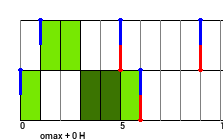
\includegraphics{figs/edfNonOptimal_EDF.png}
            \caption{A system scheduled by EDF where a deadline is missed}
            \label{fig:edfnonoptimal_edf}
        \end{center}
        \end{figure}

        However, there exists a schedule which does not miss any deadline:\\

        \begin{figure}[H]
        \begin{center}
            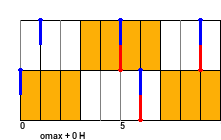
\includegraphics{figs/edfNonOptimal_PALLF.png}
            \caption{The system of Fig.~\ref{fig:edfnonoptimal_edf} with a different schedule in which no deadline is missed}
            \label{fig:edfnonoptimal_pallf}
        \end{center}
        \end{figure}

        EDF is thus non-optimal.

    \subsection{Anomalies}

        \subsubsection{Longer transitive period}
        Consider the following system

        \begin{center}
            \begin{tabular}{|r|c|c|c|c|c|}
                \hline
                            & $O_i$ & $C_i$ & $D_i$ & $T_i$ & $\alpha_i$ \\ \hline
                $\tau_1$    & 0     & 5     & 10   & 10    & 1     \\ \hline
                $\tau_2$    & 4     & 1     & 1    & 10    & 1     \\ \hline
                $\tau_3$    & 6     & 4     & 10   & 10    & 1     \\ \hline
            \end{tabular}
        \end{center}

        When scheduling this system with EDF, we see that at instant $O_{max} + 2 \cdot H$, the system has not reached a periodic behavior yet. This only happens at instant $O_{max} + 4 \cdot H$, as seen on Fig.~\ref{fig:edf_longtransitive}.\\

        \begin{figure}[H]
        \begin{center}
            \centerline{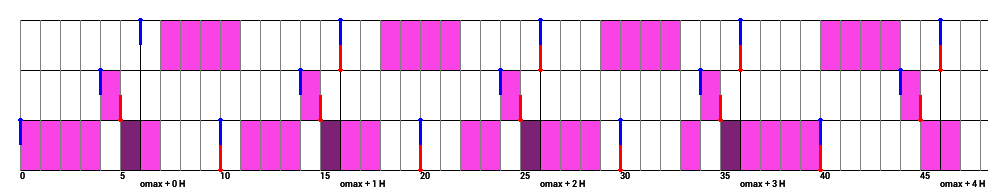
\includegraphics[width=1.4\textwidth]{figs/longTransitive2_EDF.png}}
            \caption{Scheduling of a system where the periodic behavior does not happen until $O_{max} + 4 \cdot H$}
            \label{fig:edf_longtransitive}
        \end{center}
        \end{figure}

        \subsubsection{Deadline miss in transitive, not in periodic}

    \subsection{Other properties of constrained deadline systems}

    In this section, we present other results which do not hold under the costly preemption assumption.

        \subsubsection{Idling dominate non-idling}

        Consider the following system

        \begin{center}
            \begin{tabular}{|r|c|c|c|c|c|}
                \hline
                            & $O_i$ & $C_i$ & $D_i$ & $T_i$ & $\alpha_i$ \\ \hline
                $\tau_1$    & 0     & 3     & 8    & 8     & 2     \\ \hline
                $\tau_2$    & 0     & 3     & 5    & 8     & 2     \\ \hline
                $\tau_3$    & 1     & 1     & 1    & 8     & 2     \\ \hline
            \end{tabular}
        \end{center}

        And consider the following schedule of fig.~\ref{fig:mustidle_pallf} which shows that it is feasible with an idling scheduling policy.

        \begin{figure}[H]
        \begin{center}
            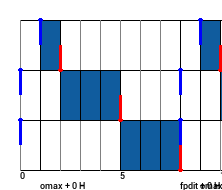
\includegraphics[scale=0.7]{figs/mustIdle_PALLF.png}
            \caption{A system scheduled by an idling algorithm. $t=0$ is an idle instant even though a job of $\tau_1$ is active}
            \label{fig:mustidle_pallf}
        \end{center}
        \end{figure}

        However, it is easy to see that no non-idling algorithm can successfully schedule this system: at $t=0$, a non-idling algorithm has to choose between $j_{1,1}$ and $j_{2,1}$ for execution, whichever is chosen will then be preempted by $j_{3,1}$ (if not, it will miss its deadline in $t=2$).\\

        Which means that at $t=2$, there will either be \mbox{$(c_{1,1} - 1) +c_{2,1} + \alpha = 7$} or \mbox{$c_{1,1} + (c_{2,1} -1) + \alpha = 7$} units of computation left to compute (including preemptions recovery) before the deadline at $t=8$, the system will thus certainly miss a deadline.


        \subsubsection{Dynamic dominate fixed-job}

        Consider the following system

        \begin{center}
            \begin{tabular}{|r|c|c|c|c|c|}
                \hline
                            & $O_i$ & $C_i$ & $D_i$ & $T_i$ & $\alpha_i$ \\ \hline
                $\tau_1$    & 0     & 4     & 8    & 8     & 1     \\ \hline
                $\tau_2$    & 0     & 1     & 5    & 8     & 1     \\ \hline
                $\tau_3$    & 3     & 1     & 1    & 8     & 1     \\ \hline
                $\tau_4$    & 5     & 1     & 1    & 8     & 1     \\ \hline
            \end{tabular}
        \end{center}

        And a successful schedule of it in Fig.~\ref{fig:dponly_pallf}.

        \begin{figure}[H]
        \begin{center}
            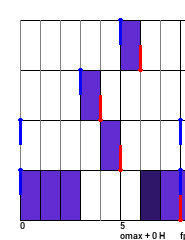
\includegraphics[scale=0.7]{figs/dponly_palff.png}
            \caption{A system scheduled by a dynamic algorithm. The priorities of $j_{1,1}$ and $j_{2,1}$ change between $t=0$ and $t=4$}
            \label{fig:dponly_pallf}
        \end{center}
        \end{figure}

        Furthermore, it can be shown that the schedule of fig.~\ref{fig:dponly_pallf} is the only successful schedule possible. However no fixed-priority algorithm (either at the task of the job level) can produce it, which shows that dynamic algorithms are necessary when considering the preemption cost.

        % \subsubsection{$u < 0.69$ is not sufficient}

        \subsubsection{Require clairvoyance}

        Consider the following the following system

        \begin{center}
            \begin{tabular}{|r|c|c|c|c|c|}
                \hline
                            & $O_i$ & $C_i$ & $D_i$ & $T_i$ & $\alpha_i$ \\ \hline
                $\tau_1$    & 22    & 2     & 2    & 24    & 1     \\ \hline
                $\tau_2$    & 0     & 5     & 12   & 12    & 1     \\ \hline
                $\tau_3$    & 4     & 5     & 6    & 12    & 1     \\ \hline
                $\tau_4$    & 9     & 1     & 1    & 24    & 1     \\ \hline
            \end{tabular}
        \end{center}

        And a successful schedule of it

        \begin{figure}[H]
        \begin{center}
            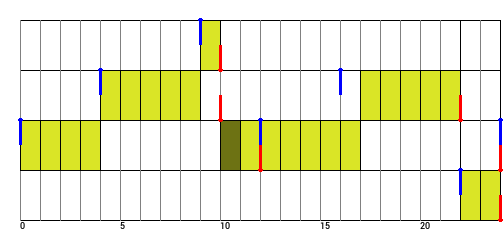
\includegraphics[scale=0.7]{figs/clairvoyance_example.png}
            \caption{A system scheduled by a clairvoyant algorithm. Different decisions have to be taken at $t=4$ and $t=16$ even though the state of the system is identical}
            \label{fig:clairvoyance}
        \end{center}
        \end{figure}


        \subsubsection{Preemption at non-arrivals}

        As we have shown previously, an optimal algorithm has to update priority of the jobs dynamically. This can be very heavy if done at each instant, and one could wonder if updating the priority only at arrivals of job would be sufficient. We show by an example that this is not the case.\\

        Consider the following system

        \begin{center}
            \begin{tabular}{|r|c|c|c|c|c|}
                \hline
                            & $O_i$ & $C_i$ & $D_i$ & $T_i$ & $\alpha_i$ \\ \hline
                $\tau_1$    & 0     & 3     & 6    & 6     & 1     \\ \hline
                $\tau_2$    & 3     & 1     & 1    & 6     & 1     \\ \hline
                $\tau_3$    & 1     & 1     & 3    & 6     & 1     \\ \hline
            \end{tabular}
        \end{center}

        And the only valid schedule of it

        \begin{figure}[H]
        \begin{center}
            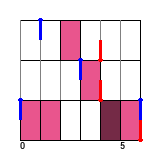
\includegraphics[scale=0.7]{figs/mpana.png}
            \caption{A valid schedule of a system. Note that the preemption occurs at $t=2$ which is not a job arrival time}
            \label{fig:mpana}
        \end{center}
        \end{figure}

        Indeed, if the preemption of $j_{1,1}$ happens at $t=1$, $j_{3,1}$ will finish its execution at $t=1$ and the instant $t=3$ will be used for a preemption recovery period which will be immediately followed by another preemption, leading to a deadline miss at $t=6$. Similarly, if $j_{1,1}$ continues its execution without preemption, either $j_{2,1}$ or $j_{3,1}$ will have to miss its deadline at $t=4$. The proposed schedule is thus the only valid and require a priority update at $t=2$.

\section{PA-EDF: an extension of EDF for costly preemption}

    In previous sections, we have shown that EDF is not optimal when including preemption costs. To the best of our knowledge, there is no known optimal algorithm in that case. This section presents an algorithm which, while not being optimal, is an improvement over the EDF algorithm.

    \subsection{Idling rule}


\nocite{*}
\bibliographystyle{plain}
\bibliography{paper-paedf}


\end{document}
